\newcommand{\startHSCdocument}[1][]{

  % Register different entries: glossary, nomenclature, acronyms
  \makeglossaries
  \hyphenation{}

  \newacronym{cpu}{CPU}{Central Processing Unit}
\newacronym{cuda}{CUDA}{Compute Unified Device Architecture}
\newacronym{gpu}{GPU}{Graphics Processing Unit}
\newacronym{ki}{KI}{Künstliche Intelligenz}
\newacronym{ppo}{PPO}{Proximal Policy Optimization}
\newacronym{relu}{ReLU}{Rectified Linear Unit}
\newacronym{gpt}{GPT}{Generative Pre-trained Transformer}
\newacronym{rl}{RL}{Reinforcement Learning}
\newacronym{api}{API}{Application Programming Interface}
  \makenomenclature
  \nomenclature[01]{\textbf{Symbol}}{\textbf{Bedeutung} \nomunit{\textbf{[phys. Einheit]}}}

  \newglossaryentry{Kästchen}
{
	name=Kästchen,
	plural=Kästchen,
	description={Ein Kästchen beschreibt ein Rechteck des Spielbretts von \textit{"Ganz schön clever"}, welches ausgefüllt werden kann, wenn bestimmte Bedingungen erfüllt sind.}
}
\newglossaryentry{Feld}
{
	name=Feld,
	plural=Felder,
	description={Ein Feld ist eines der farbigen Felder (gelb, blau, grün, orange, lila) auf dem Spielbrett von \textit{"Ganz schön clever"}.}
}
\newglossaryentry{Extra-Wahl}
{
	name=Extra-Wahl,
	plural=Extra-Wahlen,
	description={Eine Extra-Wahl beschreibt eine Wahl mithilfe des Extra-Wahl-Bonus oder vom Silbertablett eines Mitspielers.}
}
\newglossaryentry{Wahl}
{
	name=Wahl,
	plural=Wahlen,
	description={Eine Wahl beschreibt den Vorgang bei dem ein Würfel oder eine Boni gewählt wird, um eines der Kästchen auf dem Spielbrett auszufüllen.\newpage}
}
\newglossaryentry{Bonusrunde}
{
	name=Bonusrunde,
	plural=Bonusrunden,
	description={Eine Bonusrunde ist eine Runde bei der der Rundenablauf nicht wie üblich inkrementiert wird. Diese Einteilung ist notwendig, da bei Wahlen mit Boni oder vom Silbertablett eines Mitspielers andere Regeln gelten, als bei Wahlen nach dem eigenen Würfen. Alle Wahlen, bis auf Wahlen nach einem gewöhnlichen eigenen Wurf, sind Wahlen in einer Bonusrunde.}
}
\newglossaryentry{ungültige Aktion}
{
	name=ungültige Aktion,
	plural=ungültige Aktionen,
	description={Eine ungültige Aktion ist eine Aktion, die im normalen Spielablauf nicht stattfinden würde. Ungültige Aktionen treten auf, wenn dem Modell keine gültige Aktion zur Auswahl steht.}
}
\newglossaryentry{ungültiger Würfel}
{
	name=ungültiger Würfel,
	plural=ungültige Würfel,
	description={Ein ungültiger Würfel ist ein Würfel, der nicht mehr zur Wahl steht und nicht mehr geworfen wird.}
}
\newglossaryentry{Modell}
{
	name=Modell,
	plural=Modelle,
	description={Ein Modell beschreibt den Teil einer Künstlichen Intelligenz, der im Stande ist, Vorhersagen zu treffen}
}
\newglossaryentry{Agent}
{
	name=Agent,
	plural=Agenten,
	description={Ein Agent ist die ausführende Instanz der Künstlichen Intelligenz. Er nimmt die Umgebung wahr und führt Aktionen in dieser aus.}
}

  % Register actual document
  \begin{document}
  \shorthandoff{"}

  % ===========================================================================
  %                             Document header
  % ===========================================================================

  \newgeometry{
    left=2.5cm,
    right=2.5cm,
    top=2.5cm,
    bottom=2.5cm
  }

  % Correctly determine type of document and format in respective header
  \newcommand{\DocumentType}{#1}

  \begin{titlepage}
    \ifthenelse{\equal{#1}{Praxisbericht}}
      {\centering

\includegraphics[width=.8\textwidth]{framework/Logo_HS_Coburg}

\begin{Large}
  Hochschule für angewandte Wissenschaften Coburg\\
  Fakultät Elektrotechnik und Informatik\par
\end{Large}
\vspace{1.5cm}

\Large{Studiengang: \Studiengang}
\vspace{1.5cm}

\Large{Praxisbericht}
\vspace{1cm}

\huge{\Autorenname}
\vspace{1.5cm}

\begin{table}[H]
  \begin{tabular}{|L{3cm}|L{11cm}|}
  \hline
  Unternehmen & \Unternehmen        \\
              & \Abteilung          \\
              & \Strasse            \\
              & \Ort                \\
  \hline
  Zeitraum    & \Beginn \ bis \Ende \\
  \hline
  \end{tabular}
\end{table}

\large{Abgabe des Berichts: \Abgabe}

\begin{table}[H]
  \begin{tabular}{|L{3cm}|L{6cm}|L{5cm}|}
    \multicolumn{3}{l}{Freigabe zur Vorlage des Praxisberichts an der HS Coburg:} \\
    \hline
    Betreuer & \Betreuer & \\
    \hline
    Funktion & \Funktion & \textbf{\textit{Ort, Datum}}\\
    \hline
    Telefon & \Telefon & \\
    \cline{1-2}
    Email & \Email & \\
    \hline
    & & \textbf{\textit{Unterschrift Betreuer}}\\
    \hline
  \end{tabular}
\end{table}
}
      {
        \ifthenelse{\equal{#1}{Bachelorarbeit}}
          {\centering

\includegraphics[width=.8\textwidth]{framework/Logo_HS_Coburg}

\begin{Large}
  Hochschule für angewandte Wissenschaften Coburg\\
  Fakultät Elektrotechnik und Informatik\par
\end{Large}
\vspace{1.5cm}

\Large{Studiengang: \Studiengang}
\vspace{1.5cm}

\Large{\DocumentType}
\vspace{1cm}

\Huge{\Titel}
\vspace{2cm}

\huge{\Autorenname}
\vspace{2cm}

\Large{Abgabe der Arbeit: \Abgabe}

\Large{Betreut durch:}

\Large{\Betreuer, Hochschule Coburg}

\newpage
\begin{abstract}
\raggedright
Ziel dieser Arbeit war es, eine Künstliche Intelligenz, für das Brettspiel \textit{"Ganz schön clever"}, zu entwickeln und den Entwicklungs- sowie Trainingsprozess zu evaluieren.
Diese Künstliche Intelligenz wurde erfolgreich entwickelt und kann das Brettspiel \textit{"Ganz schön clever"} gut spielen. Zunächst wurde dafür ein Prototyp entwickelt, welcher dann schrittweise erweitert wurde, um die gesamte Komplexität des Spiels zu erfassen.

Das Brettspiel \textit{"Ganz schön clever"} ist ein Würfelspiel, welches eine hohe Komplexität aufweist. Diese kommt vor allem durch die vielen Aktionsmöglichkeiten des Spielers und die multiplen Zusammenhängen innerhalb des Belohnungssystems zustande. Außerdem weist es eine hohe Stochastizität auf, welche die Komplexität weiter erhöht.

Für die Implementierung der Künstlichen Intelligenz wurde Deep Reinforcement Learning verwendet. Während der Implementierungsphase kam es zunächst zu einem Problem, bei dem die Künstliche Intelligenz es nur schwer selbstständig schaffte, gültige Aktionen zu wählen, welche nicht zum Abbruch des Spiels geführt haben. Dieses Vorgehen, bei dem das Spiel nach Wahl einer ungültigen Aktion abgebrochen wurde, wurde nach einigen Tagen verworfen. Daraufhin wurde zunächst ein Verfahren implementiert, bei dem das Spiel bei ungültigen Aktionen nicht sofort abgebrochen, sondern negativ belohnt wurde. Diese Vorgehen stellte sich als gut geeignet heraus, wurde aber schnell von einem Vorgehen, welches eine Aktionsmaske verwendet abgelöst. Im Folgenden wurde eine Aktionsmaske implementiert, welche gewährleistet, dass nur gültige Aktionen gewählt werden können. Die Performanz stieg mit diesem Vorgehen von vorher durchschnittlich ungefähr 60 Prozent der Maximalpunktzahl auf 75 Prozent. Zudem ergaben sich Schwierigkeiten bei der Erweiterung des Runden-Systems und viele weitere Probleme, die behoben werden mussten.

Das Ergebnis des finalen Trainings war eine Künstliche Intelligenz, welche durchschnittlich 208 Punkte mit einer Standardabweichung von 31 im Spiel erzielt. Im Vergleich dazu erzielten menschliche Spieler in einem Test im Durchschnitt lediglich 160 Punkte.
\end{abstract}
\newpage}
          {
            \ifthenelse{\equal{#1}{Masterarbeit}}
              {\centering

\includegraphics[width=.8\textwidth]{framework/Logo_HS_Coburg}

\begin{Large}
  Hochschule für angewandte Wissenschaften Coburg\\
  Fakultät Elektrotechnik und Informatik\par
\end{Large}
\vspace{1.5cm}

\Large{Studiengang: \Studiengang}
\vspace{1.5cm}

\Large{\DocumentType}
\vspace{1cm}

\Huge{\Titel}
\vspace{2cm}

\huge{\Autorenname}
\vspace{2cm}

\Large{Abgabe der Arbeit: \Abgabe}

\Large{Betreut durch:}

\Large{\Betreuer, Hochschule Coburg}

\newpage
\begin{abstract}
\raggedright
Ziel dieser Arbeit war es, eine Künstliche Intelligenz, für das Brettspiel \textit{"Ganz schön clever"}, zu entwickeln und den Entwicklungs- sowie Trainingsprozess zu evaluieren.
Diese Künstliche Intelligenz wurde erfolgreich entwickelt und kann das Brettspiel \textit{"Ganz schön clever"} gut spielen. Zunächst wurde dafür ein Prototyp entwickelt, welcher dann schrittweise erweitert wurde, um die gesamte Komplexität des Spiels zu erfassen.

Das Brettspiel \textit{"Ganz schön clever"} ist ein Würfelspiel, welches eine hohe Komplexität aufweist. Diese kommt vor allem durch die vielen Aktionsmöglichkeiten des Spielers und die multiplen Zusammenhängen innerhalb des Belohnungssystems zustande. Außerdem weist es eine hohe Stochastizität auf, welche die Komplexität weiter erhöht.

Für die Implementierung der Künstlichen Intelligenz wurde Deep Reinforcement Learning verwendet. Während der Implementierungsphase kam es zunächst zu einem Problem, bei dem die Künstliche Intelligenz es nur schwer selbstständig schaffte, gültige Aktionen zu wählen, welche nicht zum Abbruch des Spiels geführt haben. Dieses Vorgehen, bei dem das Spiel nach Wahl einer ungültigen Aktion abgebrochen wurde, wurde nach einigen Tagen verworfen. Daraufhin wurde zunächst ein Verfahren implementiert, bei dem das Spiel bei ungültigen Aktionen nicht sofort abgebrochen, sondern negativ belohnt wurde. Diese Vorgehen stellte sich als gut geeignet heraus, wurde aber schnell von einem Vorgehen, welches eine Aktionsmaske verwendet abgelöst. Im Folgenden wurde eine Aktionsmaske implementiert, welche gewährleistet, dass nur gültige Aktionen gewählt werden können. Die Performanz stieg mit diesem Vorgehen von vorher durchschnittlich ungefähr 60 Prozent der Maximalpunktzahl auf 75 Prozent. Zudem ergaben sich Schwierigkeiten bei der Erweiterung des Runden-Systems und viele weitere Probleme, die behoben werden mussten.

Das Ergebnis des finalen Trainings war eine Künstliche Intelligenz, welche durchschnittlich 208 Punkte mit einer Standardabweichung von 31 im Spiel erzielt. Im Vergleich dazu erzielten menschliche Spieler in einem Test im Durchschnitt lediglich 160 Punkte.
\end{abstract}
\newpage}
              {
                \IfFileExists{./CustomHeader.tex}{
                  \include{CustomHeader}
                }{
                  ERROR: Please use one of the following values as parameter
                  to the HSCdocument environment:\\
                  "Praxisbericht", "Bachelorarbeit", "Masterarbeit"\\

                  To create your own document header, just create a file
                  "CustomHeader.tex" in the document root.
                }
              }
          }
      }
  \end{titlepage}

  \restoregeometry

  % ===========================================================================
  %                              Page Ordering
  % ===========================================================================

  % Set image path to "Bilder" subdirectory
  \graphicspath{{Bilder/}}

  \newpage
  \setcounter{page}{2}
  \tableofcontents

  \iftotalfigures
    \newpage
    \phantomsection
    \addcontentsline{toc}{section}{\listfigurename}
    \listoffigures
  \fi

  \iftotaltables
    \newpage
    \phantomsection
    \addcontentsline{toc}{section}{\listtablename}
    \listoftables
  \fi

  \iftotallstlistings
    \newpage
    \renewcommand{\lstlistlistingname}{Codebeispielverzeichnis}
    \phantomsection
    \addcontentsline{toc}{section}{\lstlistlistingname}
    \lstlistoflistings
  \fi

  % Nomenclature ("Symbolverzeichnis")
  \iftotalcountnomens
    \newpage
    \phantomsection
    \addcontentsline{toc}{section}{\nomname}
    \printnomenclature[1in]
  \fi

  % Acronyms
  \iftotalcountacronyms
    \newpage
    \setglossarystyle{super}
    \printglossary[type=\acronymtype,title=Abkürzungsverzeichnis]
  \fi

  \newpage
}

\newcommand{\finishHSCdocument}{
  % Bibliography
  \newpage
  \bibliographystyle{alphadin}
  \renewcommand{\refname}{Literaturverzeichnis}
  \phantomsection
  \addcontentsline{toc}{section}{\refname}
  \bibliography{Verzeichnisse/Literaturverzeichnis}

  % Glossary
  \iftotalcountglossarys
    \newpage
    \setglossarystyle{altlist}
    \printglossary
  \fi

  % Appendix
  \IfFileExists{./Sektionen/Anhang.tex}{
    \newpage
    \appendix
    \renewcommand{\thesection}{A\arabic{section}}
    \section{Code für die Attribute der Spielumgebung}
\begin{minipage}{\linewidth}
Code 17 zeigt die Klassenattribute, die für das bilden einer Punktestandhistorie relevant sind:
\vspace{0.5cm}
\begin{lstlisting}[caption={Klassenattribute für die Nachvollziehbarkeit von Punkteständen}, basicstyle=\ttfamily]
self.score
self.score_history
self.initialized
\end{lstlisting}
\end{minipage}

\begin{minipage}{\linewidth}
Code 18 zeigt die Klassenattribute der Flags für die Belohnungen der farbigen Felder. Sind diese gesetzt und sind die entsprechenden Kästchen für die Belohnung ausgefüllt, wurde die Belohnung bereits ausgeschüttet und wird es nicht erneut, bis die Attribute nach dem Spiel zurückgesetzt werden:
\vspace{0.5cm}
\begin{lstlisting}[caption={Klassenattribute für Belohnungsflags}, basicstyle=\ttfamily]
self.yellow_reward_flags = {"row": [False] * 4, "col": ...}
self.blue_reward_flags = {"row": [False] * 3, "col": ...}
self.blue_count_reward_flags = [False] * 12
self.green_reward_flags = [False] * 11
self.orange_reward_flags = [False] * 11
self.purple_reward_flags = [False] * 11
\end{lstlisting}
\end{minipage}

\begin{minipage}{\linewidth}
Code 19 zeigt die Klassenattribute für Punktestände der einzelnen farbigen Felder. Die Punktewerte werden aufaddiert, sobald Punkte im entsprechenden Feld erspielt worden sind und am Ende genutzt, um den Wert der Fuchs-Boni zu bestimmen [siehe Unterabschnitt 2.1.1]:
\vspace{0.5cm}
\begin{lstlisting}[caption={Klassenattribute für erreichte Punktestände der einzelnen farbigen Felder}, basicstyle=\ttfamily]
self.yellow_field_score
self.blue_field_score
self.green_field_score
self.orange_field_score
self.purple_field_score
\end{lstlisting}
\end{minipage}

\begin{minipage}{\linewidth}
Code 20 zeigt die Klassenattribute für die Anzahl an gewählten Kästchen in den verschiedenen farbigen Feldern. Wenn ein Kästchen in einem der Felder ausgefüllt wird, wird der Wert des entsprechenden Attributes inkrementiert. Diese Attribute dienen nicht dem Spielablauf selbst, sondern der Nachvollziehbarkeit der Strategie des Modells:
\vspace{0.5cm}
\begin{lstlisting}[caption={Klassenattribute für die Anzahl an gewählte Kästchen innerhalb der farbigen Feldern}, basicstyle=\ttfamily]
self.picked_yellow
self.picked_blue
self.picked_green
self.picked_orange
self.picked_purple
\end{lstlisting}
\end{minipage}

\newpage
\section{Pseudocode für Methoden der Implementierung}
\begin{minipage}{\linewidth}
Code 21 zeigt die Funktionsweise der Funktion zur Visualisierung der Spielumgebung (\texttt{render method}) mithilfe von Pseudocode. Die Visualisierung dient einer verbesserten Nachvollziehbarkeit der Ereignisse innerhalb der Spielumgebung:
\vspace{0.5cm}
\begin{lstlisting}[caption={Methode zur Visualisierung der Spielumgebung}]
render():
	Zeige alle relevanten Attribute und Merkmale der Umgebung an
\end{lstlisting}
\end{minipage}

\begin{minipage}{\linewidth}
Code 22 zeigt die Funktionsweise der Methode zur Generierung des Beobachtungsraumes (\texttt{\_get\_obs method}) mithilfe von Pseudocode. Diese Methode vereinfacht es, den Beobachtungsraum zu generieren, welcher jedes Mal benötigt wird, wenn ein Schritt in der Umgebung ausgeführt wird:
\vspace{0.5cm}
\begin{lstlisting}[caption={Methode zur Generierung des Beobachtungsraumes}]
_get_obs():
	Erstelle Numpy Arrays für farbige Felder
	Erstelle Numpy Array für Würfelergebnisse
	Erstelle Numpy Array für ungültige Würfel
	Füge Arraywerte für Boni und Rundenzahl hinzu
	Beobachtungsraum = Verbinde alle Arrays miteinander

	return Beobachtungsraum
\end{lstlisting}
\end{minipage}

\begin{minipage}{\linewidth}
Code 23 zeigt die Funktionsweise der Methode zur Initialisierung der Spielumgebungen (\texttt{\_init\_envs method}) mithilfe von Pseudocode. Mit dieser Methode werden Spielumgebungen initialisiert und einer Vektorumgebung zugewiesen. Diese Vektorumgebung ermöglicht es mehrere Spielumgebungen gleichzeitig zu bearbeiten. Außerdem werden Variablen für die Nachvollziehbarkeit der Abläufe innerhalb der Spielumgebung (Historien) initialisiert:
\vspace{0.5cm}
\begin{lstlisting}[caption={Methode zur Initialisierung der Spielumgebungen}]
_init_envs(Anzahl, Punktestände, Fehlversuche):
	_init():
		Spielumgebung = Initialisieren eine Spielumgebung
		Setze Aktionsmasker für die Spielumgebung
		return Spielumgebung
	Initialisiere Verktorumgebung(Anzahl, _init)
		if not Punktestände and not Fehlversuche:
			return Vektorumgebung
		if Punktestände and not Fehlversuche:
			Erstelle Variablen für Punkteständehistorie
		if not Punktestände and Fehlversuche:
			Erstelle Variablen für Fehlversuchehistorie
		if Punktestände and Fehlversuche:
			Erstelle Variablen für Punkteständehistorie
			Erstelle Variablen für Fehlversuchehistorie
	return Vektorumgebung, Variablen für Historien
\end{lstlisting}
\end{minipage}

\begin{minipage}{\linewidth}
Code 24 zeigt die Funktionsweise der Methode zum Anwenden der Aktionsmaske (\texttt{mask\_fn method}) mithilfe von Pseudocode. Die Methode dient dazu dem Modell die Aktionsmasken der einzelnen Spielumgebungen zu übergeben:
\vspace{0.5cm}
\begin{lstlisting}[caption={Methode zum Anwenden der Aktionsmaske}]
mask_fn(Spielumgebung):
	Caste Spielumgebung in benutzerdefinierte Spielumgebung
	return Aktionsmaske der Spielumgebung
\end{lstlisting}
\end{minipage}

\begin{minipage}{\linewidth}
Code 25 zeigt die Funktionsweise der Methoden zum Erstellen von Einträgen und Historien (\texttt{make\_fail\_entries method, make\_score\_entries method, make\_fail\_history\_entry method, make\_score\_history\_entry method}) mithilfe von Pseudocode. Diese Methoden erstellen Einträge und Historien von erzielten Punkteständen und der Anzahl getätigter ungültiger Aktionen innerhalb abgeschlossener Spiele:
\vspace{0.5cm}
\begin{lstlisting}[caption={Methoden zum Erstellen von Einträgen für Historien}]
make_fail_entries(Punktebelohnungen, Anzahl, Fehlversuche):
	if Punktebelohnung < 0:
		Inkrementiere Fehlversuche der Umgebung

make_score_entries(Punktebelohnungen, Anzahl, Punktestände):
	if Punktebelohnung > 0:
		Addiere Punktebelohnung zum Punktestand der Umgebung

make_fail_history_entry(Fehlversuche, Fehlversuchshistorie)
	if Umgebung terminiert:
		Hänge Fehlversuche an Fehlversuchshistorie an

make_score_history_entry(Punktestände, Punktehistorie)
	if Umgebung terminiert:
		Hänge Punktestand der Umgebung Punktehistorie an
\end{lstlisting}
\end{minipage}

\begin{minipage}{\linewidth}
Code 26 zeigt die Funktionsweise der Methode zum Plotten von Historien (\texttt{plot\_history method}) mithilfe von Pseudocode. Diese Methode visualisiert die generierten Historien:
\vspace{0.5cm}
\begin{lstlisting}[caption={Methode zum Plotten von Historien}]
plot_history(Historie):
	Plotte jeden Eintrag der Historie
	Setze Titel
	Setze Labels
	Zeige Grafik an
\end{lstlisting}
\end{minipage}
  }{}

  % Declaration of Honor
  \newpage
  \phantomsection
  \addcontentsline{toc}{section}{Ehrenwörtliche Erklärung}
  \lhead{Ehrenwörtliche Erklärung}
  \thispagestyle{empty}

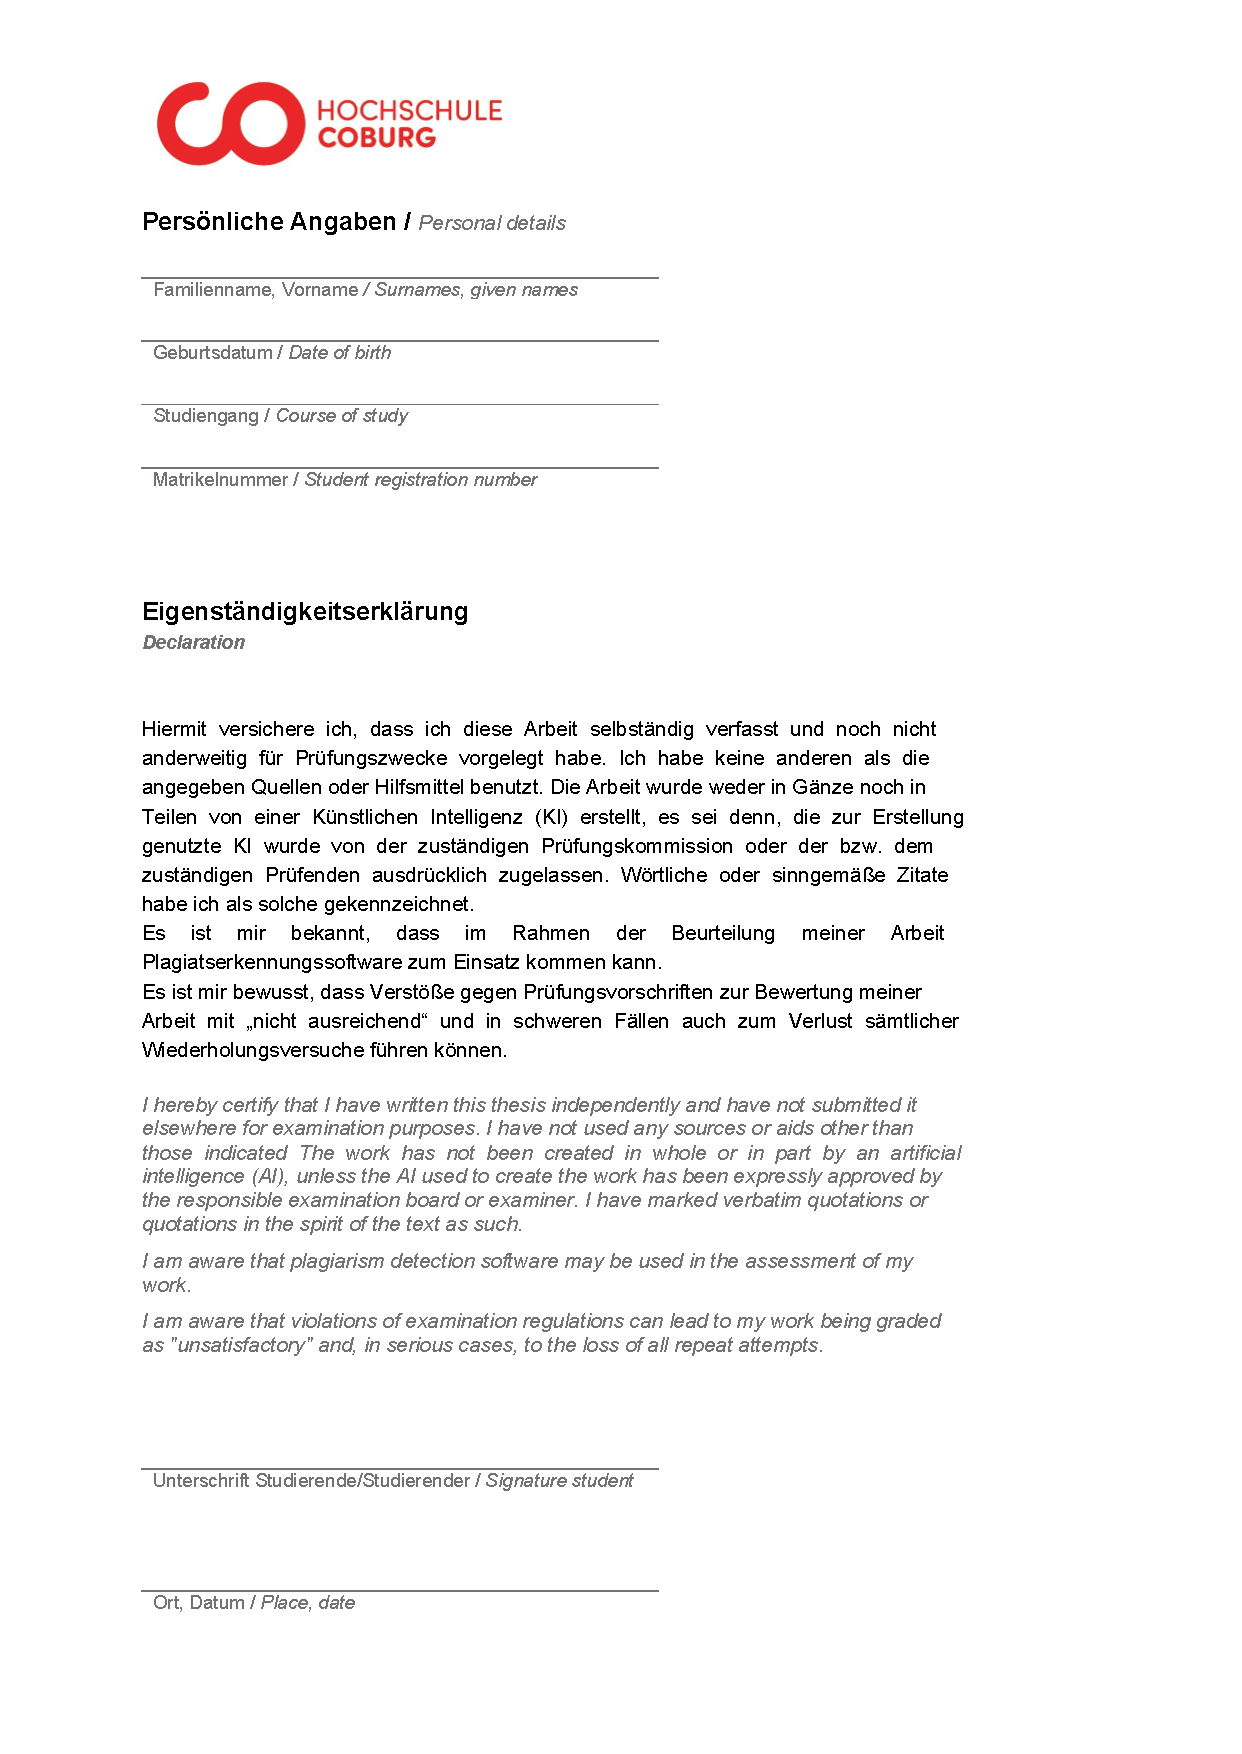
\includepdf[
  pages=-,
  pagecommand={},
  picturecommand*={
    \put(75,714){\large \Autorenname}
    \put(75,683){\large \Geburtsdatum}
    \put(75,652){\large \Studiengang}
    \put(75,622){\large \Matrikelnummer}
    \put(75,81.5){\large \Ort, den \today}
  }
]{framework/_Declaration_of_Honor.pdf}


  % TODO list
  \iftotalcounttodos
    \listoftodos[TODOs]
  \fi

  \end{document}
}

% ===========================================================================
%                   Simplified centered & colored tables
% ===========================================================================

\newenvironment{colortable}[1]{
  \begin{center}
    \begin{tabular}{#1}
    \hline
    \rowcolor{Gray}
}
{
    \hline
    \end{tabular}
  \end{center}
}

\newcommand{\tablecontent}{
  \hline
  \rowcolor{White}
}
